\chapter{CHAPTER 2 TITTLE}
\label{ch:relatedwork}

Lorem ipsum dolor sit amet, consectetur adipiscing elit. Nam in venenatis ligula, eget congue turpis. Praesent ante quam, facilisis at magna sed, lacinia iaculis eros. Aenean id dui augue. Aenean in nibh sollicitudin erat accumsan venenatis id eget magna. Maecenas in metus lorem. Pellentesque id accumsan urna, faucibus volutpat arcu. Fusce tempor lectus quis purus accumsan malesuada.

Citation examples: networkX \cite{SciPyProceedings_11}, scikit-learn \cite{scikit-learn}, and Spectral Clustering tutorial \cite{von2007tutorial}.


\section*{Section 1} 
\addcontentsline{toc}{section}{Section 1}

Curabitur vel nisi aliquam, faucibus est sed, semper mi. Praesent eget suscipit lacus. Maecenas fringilla erat vitae tortor imperdiet, eu interdum est molestie. Sed aliquet interdum magna non venenatis. Proin ut elit porta, tincidunt mauris quis, condimentum mauris. Sed in nisi non sem fringilla pharetra. Sed lacinia convallis libero a ultricies. Curabitur varius blandit dui. Cras tempus dignissim elementum. Sed nisl libero, efficitur et nisl nec, fringilla varius libero. Aenean eu dictum nunc, ac convallis turpis. Donec convallis tortor in lectus rhoncus, ac laoreet arcu convallis. Phasellus at magna interdum, mattis tellus vitae, varius sapien. Pellentesque auctor neque ante, sit amet posuere nibh cursus vel. Phasellus sed lacinia leo. 


\subsection*{Subsection 1} 


Lorem ipsum dolor sit amet, consectetur adipiscing elit. Ut sed est bibendum, vestibulum enim ac, mattis turpis. Maecenas blandit dui a dui fermentum venenatis. Maecenas posuere augue sed porttitor posuere. Donec vitae tortor faucibus, luctus urna vitae, hendrerit massa. Cras ac dui dui. Etiam euismod vehicula metus, sit amet ultricies massa blandit vitae. Aliquam sodales tempor lorem, ac venenatis diam convallis id. Maecenas ornare vulputate tellus et volutpat. Fusce vehicula nisi ac lorem varius bibendum. Pellentesque viverra ultricies libero, a malesuada augue ultricies nec.

Table~\ref{tab:table2} shows...


\begin{table}[ht]
\caption[Second table phasellus at magna interdum, mattis tellus vitae, varius sapien pellentesque auctor neque ante, sit amet posuere nibh cursus vel]
{Second table phasellus at magna interdum, mattis tellus vitae, varius sapien pellentesque auctor neque ante, sit amet posuere nibh cursus vel. Phasellus sed lacinia leo. Only the first sentence of the images and tables should show up in the tables of contents.}
\centering
\fontsize{10}{12}\selectfont
\begin{tabular}{|l|r|r|}
\hline
Dataset name & Number of records  & Number of users \\
\hline 
Dataset A & 248 & 20 \\
\hline
Dataset B & 464 & 28 \\
\hline
Dataset C & 348 & 7 \\
\hline
Dataset D & 419 & 5\\
\hline
Dataset E & 854 & 15\\
\hline
\end{tabular}
\label{tab:table2}
\end{table}


Lorem ipsum dolor sit amet, consectetur adipiscing elit. Ut sed est bibendum, vestibulum enim ac, mattis turpis. Maecenas blandit dui a dui fermentum venenatis. Maecenas posuere augue sed porttitor posuere. Donec vitae tortor faucibus, luctus urna vitae, hendrerit massa. Cras ac dui dui. Etiam euismod vehicula metus, sit amet ultricies massa blandit vitae. Aliquam sodales tempor lorem, ac venenatis diam convallis id. Maecenas ornare vulputate tellus et volutpat. Fusce vehicula nisi ac lorem varius bibendum. Pellentesque viverra ultricies libero, a malesuada augue ultricies nec.

\subsection*{Subsection 2} 

Lorem ipsum dolor sit amet, consectetur adipiscing elit. Ut sed est bibendum, vestibulum enim ac, mattis turpis. Maecenas blandit dui a dui fermentum venenatis. Maecenas posuere augue sed porttitor posuere. Donec vitae tortor faucibus, luctus urna vitae, hendrerit massa. Cras ac dui dui. Etiam euismod vehicula metus, sit amet ultricies massa blandit vitae. Aliquam sodales tempor lorem, ac venenatis diam convallis id. Maecenas ornare vulputate tellus et volutpat. Fusce vehicula nisi ac lorem varius bibendum. Pellentesque viverra ultricies libero, a malesuada augue ultricies nec.



Figure~\ref{fig:figure2} shows...

\begin{figure}[h!]
\centering
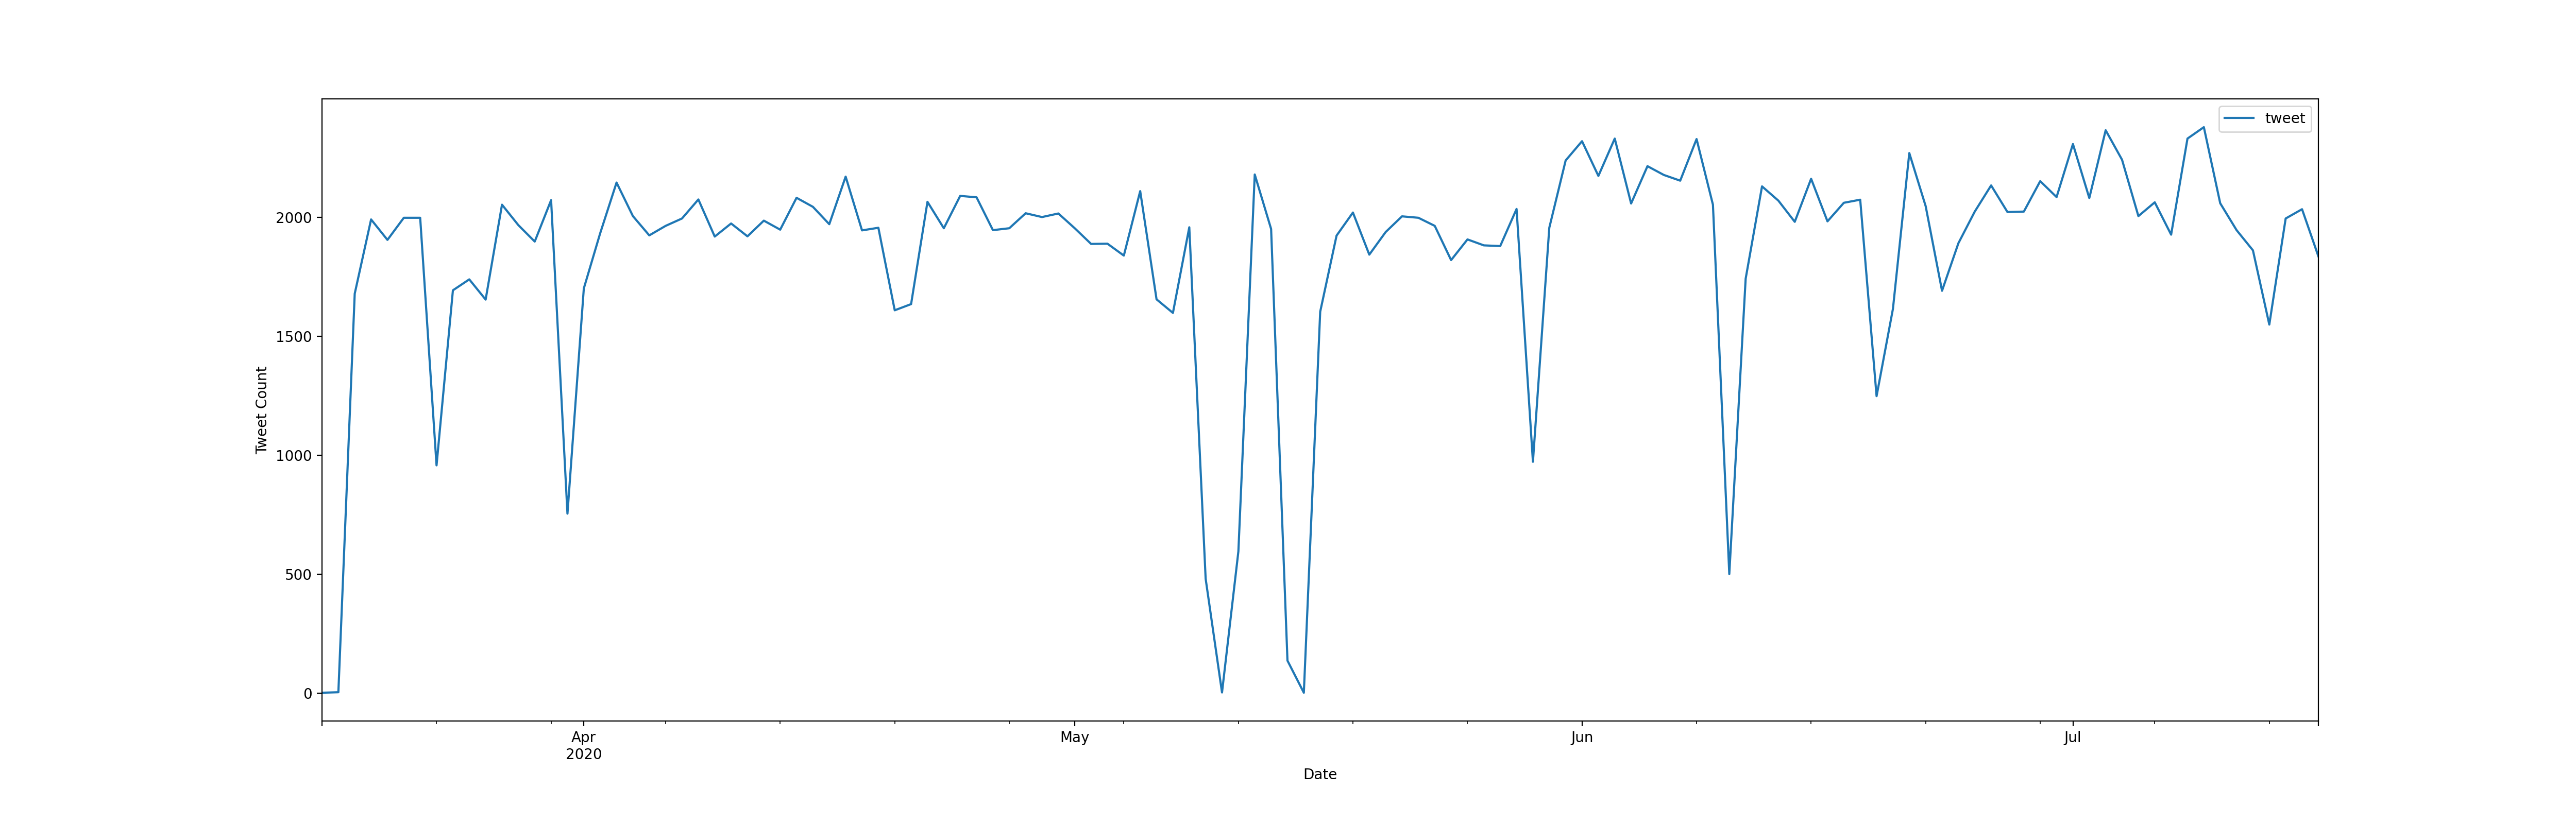
\includegraphics[scale=0.3]{Figs/Fig2.png}
\caption[Second image phasellus at magna interdum, mattis tellus vitae, varius sapien pellentesque auctor neque ante]
{Second image phasellus at magna interdum, mattis tellus vitae, varius sapien pellentesque auctor neque ante. Phasellus sed lacinia leo. Only the first sentence of the images and tables should show up in the tables of contents.}
\label{fig:figure2}
\end{figure}


\section*{Section 2} 
\addcontentsline{toc}{section}{Section 2}

Lorem ipsum dolor sit amet, consectetur adipiscing elit. Ut sed est bibendum, vestibulum enim ac, mattis turpis. Maecenas blandit dui a dui fermentum venenatis. Maecenas posuere augue sed porttitor posuere. Donec vitae tortor faucibus, luctus urna vitae, hendrerit massa. Cras ac dui dui. Etiam euismod vehicula metus, sit amet ultricies massa blandit vitae. Aliquam sodales tempor lorem, ac venenatis diam convallis id. Maecenas ornare vulputate tellus et volutpat. Fusce vehicula nisi ac lorem varius bibendum. Pellentesque viverra ultricies libero, a malesuada augue ultricies nec.


